\section{Proposed Artificial Neural Network Archicteture}\label{sec:design-ANN}
This section proposes an artificial neural network architecture (ANN), to be used in this project.
Modern approaches to autonomous driving often involves a type of ANN called deep neural networks (DNN), specifically convolutional neural networks (CNN), for tasks relating to computer vision, such as lane following and other decision making based off of image data.
\cite{yang_end--end_2018, patil_convnets_2019, kocic_end--end_2019, bojarski_end--end-nvidea_2016, nain_efficientnet_2019, zhang_yolo--v3_2018}

Designing an artificial neural network from scratch is a time consuming endeavour in itself, involving many subsequent evaluations of the models, using training data to arrive at a satisfactory model.
For the purpose of this project, this would be out of scope, but fortunately several models used for autonomous driving have already been designed \cite{bojarski_end--end-nvidea_2016, kocic_end--end_2019, zhang_yolo--v3_2018}.
One of the popular ones, are the Nvidea model, also called PilotNet, which has been used for real life applications as well as for projects in artificial settings such as this.
For this project PilotNet is proposed as the vantage point for the convolutional neural network architecture.

\begin{figure} [H]
    \centering
    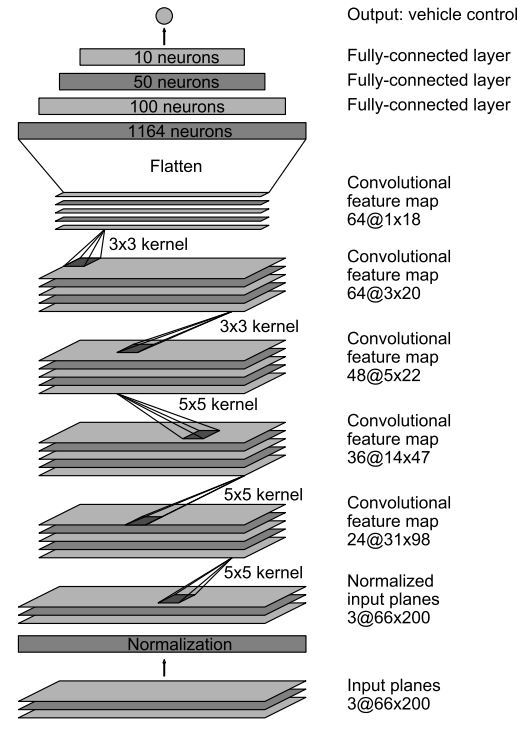
\includegraphics[scale=0.8]{design/nvidea_model_architecture.JPG}
    \caption{Diagram of the neural network architecture of PilotNet \cite{bojarski_end--end-nvidea_2016}}
    \label{fig:design-ANN-nvideaModel}
\end{figure}

PilotNet utilizes a CNN with a normalization layer, 5 convolutional layers and 3 fully connected layers, which can be seen in \autoref{fig:design-ANN-nvideaModel}.
The inputs are images, 3 channels deep, with a width of 200 and height of 66, which can be adjusted depending on the needs for the image size.
The 3 channels are YUV, as opposed to RGB \footnote{YUV is a different color space encoding than RGB that divides the image into a brightness component (Y) and a blue projection (U) and red projection (V), it is more efficient than RGB and comparably reduces the bandwidth, which is why most videocards render images using YUV directly \cite{wikipeadia_yuv_2019, sensorray_rgb--vs--yuv_2019}.
}\todo{maybe better source than wiki}.
These images are normalized before feeding them into the network.
The filters for the convolutional layers are 5x5 kernels for the first three convolutions with a stride of 2x2 and 3x3 for the last two convolutions, with no stride.
Finally the network is flattened, to acommodate dimensionality of the three fully connected layers in the end, resulting in a singular output, that is the steering angle for the car.
\cite{bojarski_end--end-nvidea_2016}

For purposes of saving time, this architecture is the point of departure for this project, however it will be subject to a few changes, which will be described in \autoref{ch:impl}.
\todo{Ensure this fits with the changes made if any}
